\subsection{Scenario 2: Alternative solution selection} \label{val-as}
The goal of the alternative solution selection scenario is to validate if the decision design pattern can help software product managers with evidence-based alternative solution selection.

\begin{center}
\large\color{document}{\valtwo} 
\end{center}

A software product manager needs to select the best solution\footnote{A solution is equal to a behavioural goal.} to contribute to a combination of soft goals. The right solution balances the importance of soft goals. This balance results in a solution that addresses the soft goals considering their importance. The wrong solution will be unbalanced and soft goals that are less important might be addressed to a larger extent compared to soft goals of higher importance.

\subsubsection{Decision ontology pattern}
Table \ref{table:as_formal_dataproperties} presents the knowledge criteria, based on the description in section \ref{tf-val-as} \nameref{tf-val-as}, that a software product manager uses to decide which solution fits best to the defined soft goals and their importance. We define the $Soft\_Goal$, $Behavioural\_Goal$, and $Score$ classes as decision-relevant \emph{root} classes. $So{\f}t\_Goal$ and $Behavioural\_Goal$ are a sub-class of $Goal$. We need the $System$ class to provide the context of the soft goals and for the reproduction of information. Figure \ref{fig:as-ont} presents the alternative solution selection ontology.  

\begin{figure}[H]
\centering
  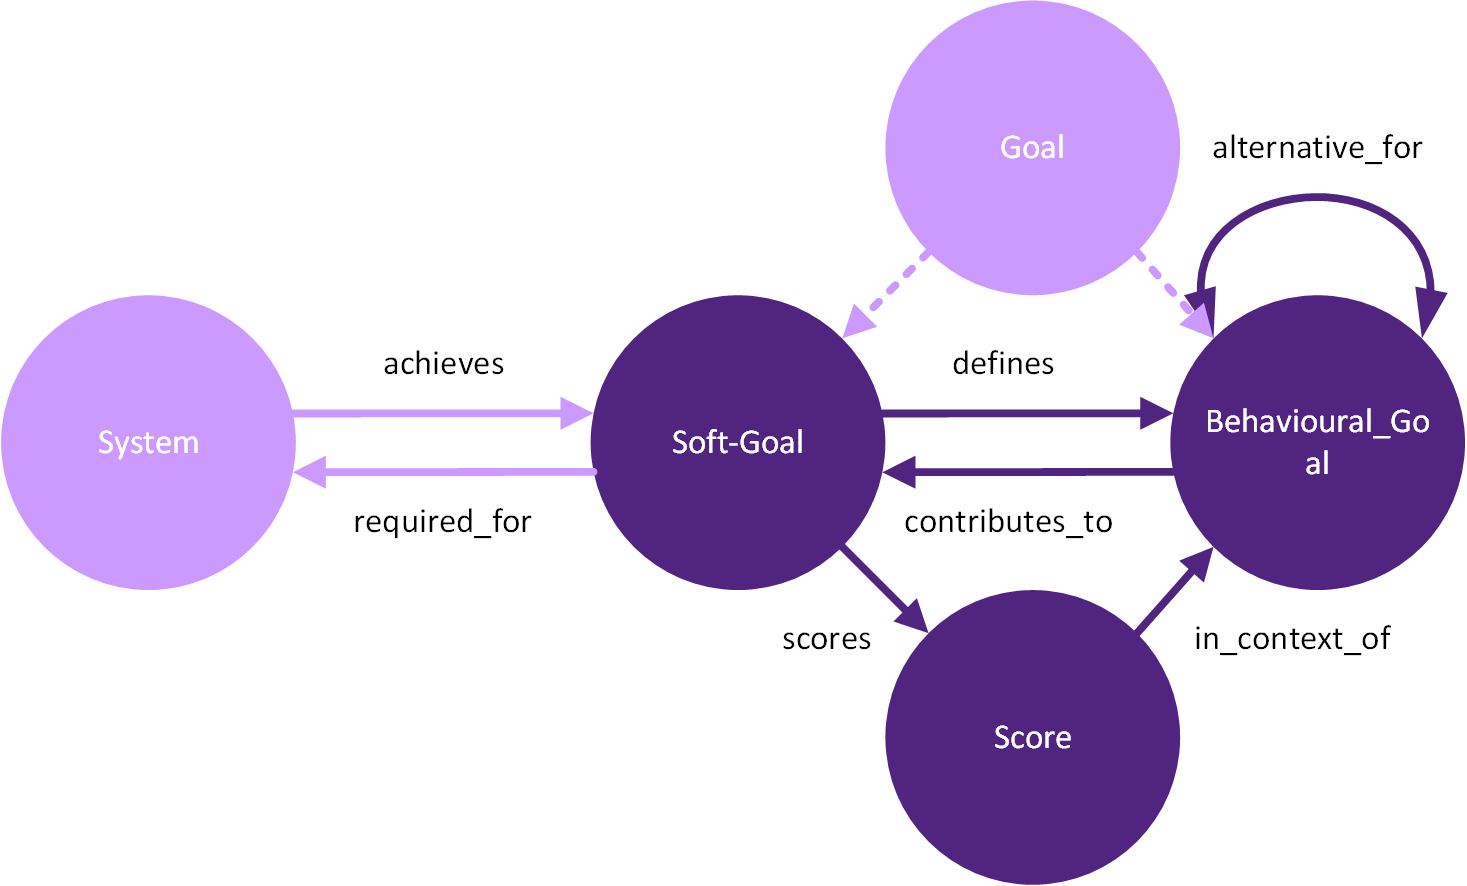
\includegraphics[width=12cm]{../../Images/05_Validation/05_ONT_AS.png}
  \caption{The alternative solution selection ontology. The \textcolor{Violet}{violet} nodes represent the decision-relevant root classes. The  \textcolor{LightViolet}{light violet} nodes represent the classes we need for the reproduction pattern.}
  \label{fig:as-ont}
\end{figure}

The $scores$ and $in\_context\_of$ object properties are essential for the structural integrity of the ontology. We use them to infer the behavioural goals that contribute to a $So{\f}t\_Goal$. A $So{\f}t\_Goal$ that does not define at least one $Behavioural\_Goal$ leads to structural problems. Missing the $contributes\_to$ object property influences the reliability of the information that we present in the dashboards.

\subsubsection{Instantiation of the decision ontology pattern}
The instantiation of the decision ontology pattern for alternative solution selection follows the same steps as the instantiation of the decision ontology pattern for requirements prioritisation. We need to instantiate the knowledge criteria and motivate, for each knowledge criterion, the information we need to reproduce the knowledge criterion. Table \ref{table:as_formal_dataproperties} presents the knowledge criteria that a software product manager needs to understand to select the right solution.

We modify equation \ref{eq:totalScore} in a way the definitions fit the alternative solution selection knowledge criteria. Equation \ref{eq:totalScore1} presents the modified equation in which $bg$ represents an individual classified as a $Behavioural\_Goal$, and $sg$ represents an individual classified as a $So{\f}t\_Goal$.

\begin{equation} \label{eq:totalScore1}
totalScore(bg)=\sum_{soft\text{-}goal} (contribution(bg,sg) \times weighted\_significance(sg))
\end{equation}

We define the contribution and weighted significance as knowledge criteria and add them to the domain of the $So{\f}t\_Goal$ and $Score$ classes of the alternative solution selection ontology. We define the completeness-level of a $So{\f}t\_Goal$ and $Score$ based on the knowledge criteria. 

\begin{table}[H]
\centering
\caption{An overview of the formal knowledge criteria that alternative solution selection needs.}
\begin{tabular}{| p{8cm} | p{4cm} | }
\hline
\rowcolor{document}
\color{documentText}Data Property & \color{documentText}Domain  \\
\hline
$so{\f}t\_goal\_weighted\_significance$ & $So{\f}t\_Goal$  \\
\hdashline
$score\_contribution$ & $Score$ \\
\hline
\end{tabular}
\label{table:as_formal_dataproperties}
\end{table}

The motivation for the reproducibility of the knowledge criteria follows a similar argumentation as we presented the validation of the requirements prioritisation scenario. We have selected the $system\_objective$, $system\_as\_is$, $system\_to\_be$, and $goal\_objective$ as background information for the $So{\f}t\_goal\_weighted\_significance$. Additionally, we have selected the $goal\_objective$ as background information for the $score\_contribution$.

\subsubsection{Instantiation overview}
We combine the alternative solution selection ontology and the decision ontology pattern. The decision ontology pattern validates that the individuals classified as $In{\f}ormation$ and the information types that are subclasses of $In{\f}ormation$ are evidence-based. Figure \ref{fig:05_AS_Instantiated} presents a conceptual overview of the instantiation. We have summarized the information types in three main information classes: $Score\_*$ includes the information classes related to the score, $Goal\_*$ includes the information classes related to the goal, and $System\_*$ includes the information classes related to the system. 

\begin{figure}[H]
\centering
  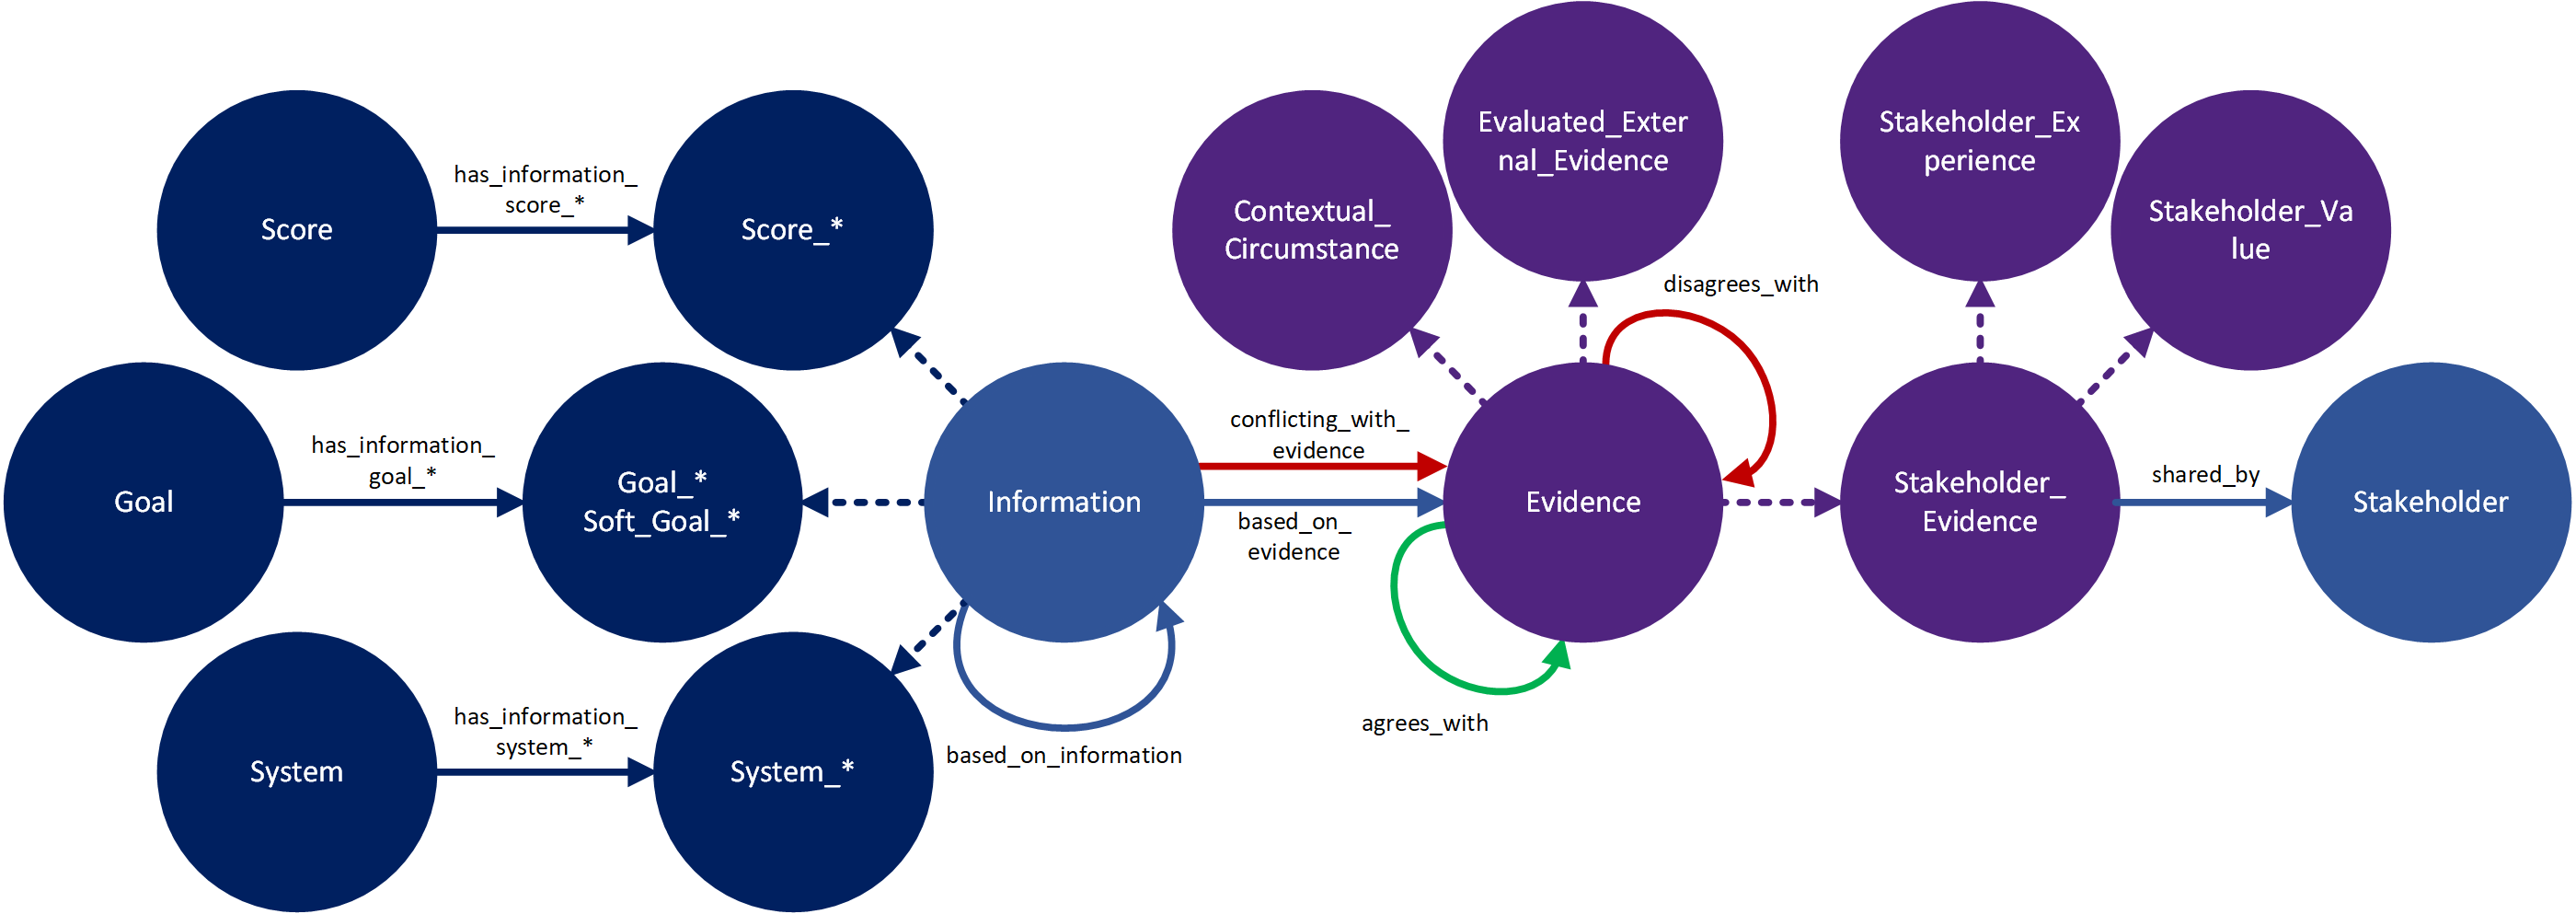
\includegraphics[width=17cm]{../../Images/05_Validation/05_AS_Instantiated.png}
  \caption{The combined alternative solution selection ontology and the decision design pattern ontology.}
  \label{fig:05_AS_Instantiated}
\end{figure}

\subsubsection{Structural validation}
The structural validation prevents an incorrect information maturity-level. An incorrect maximum number of violations causes an incorrect information maturity-level. The structural violations are not part of the functions that define the information maturity-level. Two scenarios can cause an incorrect maximum number of violations:
\begin{enumerate}
\item The sum of the weighted significance of the soft goals related to one system is not equal to the total relative weight. This situation might mean a soft goal is missing, there are too many soft goals, or the values are incorrect.
\item Each behavioural goal should have at least one alternative. If this is not the case, the decision-maker has no decision to make.
\end{enumerate}

If the reasoner finds structural violations, the dashboards are not reliable and will not show up. The decision-maker needs to solve the structural violations first.

\paragraph{Structural validation: the sum of the weighted significance}
The sum of the weighted significances of the soft goals required for one system needs to be equal to an arbitrary fixed number, for example, $10$. This fixed number forces the decision-maker to weigh the value of the soft goals against each other. We continue to use $10$ as an example throughout the validation of the alternative solution selection scenario. Code sample \ref{SPARQL_AS_WS} presents a SPARQL query embedded in a SHACL constraint\footnote{We removed the declared prefixes from code sample \ref{SPARQL_AS_WS}. The full source code is available in our GitHub repository.}. The SPARQL query finds a list of systems and their total weighted significance by summing up the weighted significances of the soft goals related to the $System$. The $HAVING$ statement filters out systems with a weighted significance that does not equal $10$. As a result, the output of the SPARQL query lists the systems that have a weighted significance that does not equal $10$. The SHACL shape that embeds the SPARQL query generates a violation on each of those systems.

\begin{lstlisting}[float,language=SHACLSPARQL,caption={A SPARQL query embedded in a SHACL shape. The SHACL shape generates violations depending on the outcome of the SPARQL query.},label={SPARQL_AS_WS}][H]
as:SoftGoalWeightedSignificanceShape
	sh:targetClass as:System ;
	sh:sparql [
		sh:message "Structural: ensure the weighted significance of this soft_goal equals to 10." ;
		sh:prefixes _:prefixes ;
		sh:select """
			SELECT $this (SUM(?dv) as ?totalws)
			WHERE
			{
					?sg as:has_information_soft_goal_weighted_significance ?ws .
					?ws as:data_value ?dv .
					$this as:achieves ?sg .
			}
			GROUP BY $this 
			HAVING (SUM(?dv) != 10)
		""" ;
	] .
\end{lstlisting}

\paragraph{Structural validation: behavioural goals}
The software product manager needs to select the best behavioural goal that addresses the soft goals considering their weighted significance. Therefore, each $Behavioural\_Goal$ should have at least one alternative. Code sample \ref{SHACL_AS_STRUC_BG} presents the SHACL shape that generates a violation if an individual that is classified as $Behavioural\_Goal$ violates this constraint.

\begin{lstlisting}[float,language=SHACL,caption={The SHACL shapes that generate a violation if an individual that is classified as $Behavioural\_Goal$ violates this constraint.},label={SHACL_AS_STRUC_BG}][H]
as:BehaviouralGoalShape a sh:NodeShape;
	sh:targetClass as:Used_Behavioural_Goal; 
	sh:property [
		sh:path as:alternative_for;
		sh:severity sh:Violation; 
		sh:minCount 1; 
		sh:message "Structural: add at least one alternative for this behavioural goal."; ].
\end{lstlisting}

\subsubsection{Test scenarios for the decision ontology pattern}
We define six abstract test scenarios. The abstraction makes it easier to validate that a specific scenario triggers the expected violations. Scenario $SC0$ validates the structure of the ontology. The first scenario ($SC1$) should not generate any violations. The other scenarios validate a specific pattern and are structurally valid. This structure limits the complexity of the scenarios and their outcomes. 

Scenario $SC0$ deviates from the requirements prioritisation scenarios while we have similarly validated the other scenarios. Therefore, we describe $SC0$, including the sample data, in detail, while we summarise the results of the other scenarios in table \ref{table:as_number_of_violations}.

\paragraph{Scenario 0 ($SC0$): Structural validation}
The structural validation needs to ensure that each $Behavioural\_Goal$ has at least one alternative and that the sum of the weighted significance of the soft goals related to a system equals $10$. 

We create $Behavioural\_Goal\_SC00$ without any alternatives. Figure \ref{fig:05_AS_SC0_Behavioural_Goal_SC00} presents $Behavioural\_Goal\_SC00$ in Prot\'eg\'e and confirms the lack of alternatives by not showing an $alternative\_{\f}or$ object property.

\begin{figure}[H]
\centering
  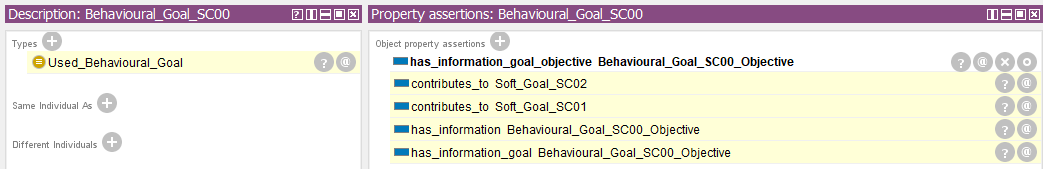
\includegraphics[width=13cm]{../../Images/05_Validation/05_AS_SC5_Behavioural_Goal_SC00.png}
  \caption{$Behavioural\_Goal\_SC00$ in Prot\'eg\'e.}
  \label{fig:05_AS_SC0_Behavioural_Goal_SC00}
\end{figure}

Additionally, we create $System\_SC0$ with two soft goals: $So{\f}t\_Goal\_SC01$ and $So{\f}t\_Goal\_SC02$. We set the weighted significance of $So{\f}t\_Goal\_SC01$ to $3$ and of $So{\f}t\_Goal\_SC02$ to $4$. The sum of the weighted significance of the soft goals contributing to $System\_SC0$ is $7$. Figures \ref{fig:05_AS_SC0_SoftGoal_SC01} and \ref{fig:05_AS_SC0_SoftGoal_SC02} present $So{\f}t\_Goal\_SC01$ and $So{\f}t\_Goal\_SC02$ in Prot\'eg\'e.

\begin{figure}[H]
\centering
  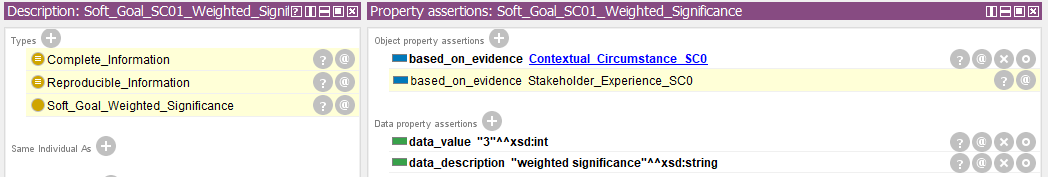
\includegraphics[width=15cm]{../../Images/05_Validation/05_AS_SC0_SG_SC01.png}
  \caption{$So{\f}t\_Goal\_SC01$ in Prot\'eg\'e.}
  \label{fig:05_AS_SC0_SoftGoal_SC01}
\end{figure}

\begin{figure}[H]
\centering
  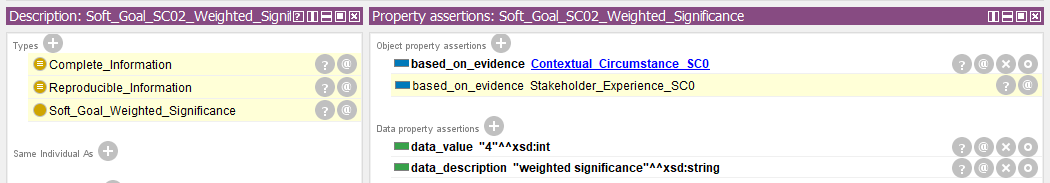
\includegraphics[width=15cm]{../../Images/05_Validation/05_AS_SC0_SG_SC02.png}
  \caption{$So{\f}t\_Goal\_SC02$ in Prot\'eg\'e.}
  \label{fig:05_AS_SC0_SoftGoal_SC02}
\end{figure}

\paragraph{The result of the test scenarios}
Table \ref{table:as_number_of_violations} presents the results of the tests. We detect $38$ violations for the decision ontology pattern. Figure \ref{fig:RP_AS_Results} presents an extract of the results as the SHACL4P plugin presents them in Prot\'eg\'e.

\begin{table}[H]
\centering
\caption{The number of expected and detected violations per scenario and pattern.}
\begin{tabular}{| p{3cm} | p{3cm} | p{4cm} | p{4cm} | }
\hline
\rowcolor{document}
\color{documentText}Scenario & \color{documentText}Scenario & \color{documentText}Expected violations & \color{documentText}Detected violations  \\
\hline
$SC0$ & Structural & 2 & 2 \\
\hdashline
$SC2$ & n/a & 0 & 0 \\
\hdashline
$SC2$ & Completeness & 12 & 12 \\
\hdashline
$SC3$ & Reproducibility & 4 & 4 \\
\hdashline
$SC4$ & Conflict & 18 & 18 \\
\hdashline
$SC5$ & Consensus & 2 & 2 \\
\hline
\end{tabular}
\label{table:as_number_of_violations}
\end{table}

\begin{figure}[H]
\centering
  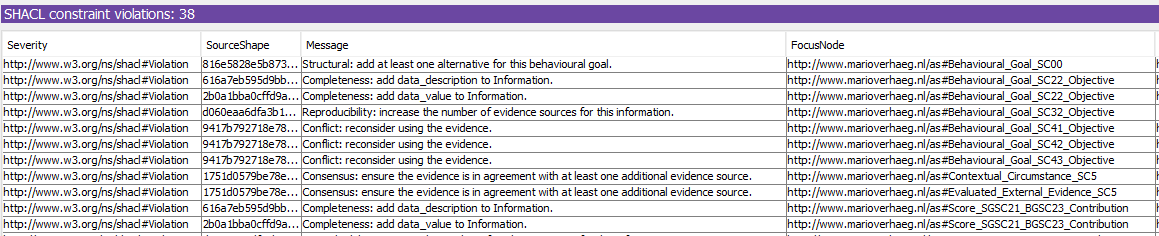
\includegraphics[width=17cm]{../../Images/05_Validation/05_AS_SC_Results.png}
  \caption{An extract of the results as the SHACL4P plugin presents them in Prot\'eg\'e.}
  \label{fig:RP_AS_Results}
\end{figure}

\subsubsection{Decision-relevant root individuals}
We determine the decision-relevant root individuals for an alternative solution selection decision. The alternative solution selection decision typically starts with a behavioural goal $bg$. This behavioural goal solves a specific problem. The software product manager wants to know if there are alternatives for this behavioural goal and to what extent this behavioural goal addresses the soft goals. Code sample \ref{SPARQL_AS_VAL_Related} presents a SPARQL query that retrieves the system, the soft goals, the contributing behavioural goals, and the scores using parameter $<bg>$. We execute the SPARQL query and feed the result into the set $RI$. We define function $asri(bg) = RI$ to logically represent the SPARQL query. 

\begin{lstlisting}[float,language=SPARQL1,caption={A SPARQL query that retrieves the system, the required soft goals, contributing behavioural goals, and scores using parameter $<bg>$.},label={SPARQL_AS_VAL_Related}][H]
SELECT DISTINCT ?ri
WHERE 
{
	# Gather systems
	{
		?sg as:defines ?bg .
		?ri as:achieves ?sg .		
	}
	UNION
	# Gather soft goals
	{
		?ri as:defines ?bg .
	}
	UNION
	# Gather scores
	{
		?bg as:alternative_for ?bga .
		?ri as:in_context_of ?bga .
	}
	UNION
	# Gather behavioural goals
	{
		?bg as:alternative_for ?ri .
	}
	FILTER(?bg = as:Behavioural_Goal_SC21)
}
\end{lstlisting}

\subsubsection{Test scenarios for the decision presentation pattern}
We use one behavioural goal to validate the decision presentation pattern for alternative solution selection. The software product manager is interested in $Behavioural\_Goal\_SC21$ and wants to understand its alternatives and, eventually, select the right solution. 

\paragraph{Decision $DEC1$: $Behavioural\_Goal\_SC21$}
A software product manager needs to decide if $Behavioural\_Goal\_SC21$ is the right solution considering the soft goals and their significant weights. The first question we ask is:

\begin{center}
\large\color{document}{Is the information ready for this decision?}
\end{center}

The first dashboard of the decision presentation pattern helps a decision-maker to answer this question. We define the consolidated information maturity-level, and the evidence spread for $Behavioural\_Goal\_SC21$ to generate this dashboard.

We use function $asri(Behavioural\_Goal\_SC21)$ to define $RI_{DEC1}$. $RI_{DEC1}$ is the set of decision-relevant root individuals. $RI_{DEC1}$ includes the individuals' table \ref{table:as_maximum_evidence_dec1} presents. Table \ref{table:as_maximum_evidence_dec1} also presents the maximum and the actual number of violations per decision-relevant root individual. The bottom line of the table presents the maximum and the actual number of violations per pattern. We conclude that decision $DEC1$ can generate up to $97$ violations. We conclude that decision $DEC1$ generates $12$ completeness violations. 

\begin{table}[H]
\centering
\caption{The maximum number of violations per decision-relevant root individual.}
\begin{tabular}{| p{4cm} | p{0.7cm} | p{0.7cm} | p{0.7cm} | p{0.7cm} | p{1.2cm} | p{0.7cm} | p{0.7cm} | p{0.7cm} | p{0.7cm} | p{1.1cm} |}
\hline
\rowcolor{document}
\color{documentText}Function & \color{documentText}$mvi_1$ & \color{documentText}$mvi_2$ & \color{documentText}$mvi_3$ & \color{documentText}$mvi_4$ & \color{documentText}$Total_{mv}$ & \color{documentText}$avi_1$ & \color{documentText}$avi_2$ & \color{documentText}$avi_3$ & \color{documentText}$avi_4$ & \color{documentText}$Total_{av}$ \\
\hline
$System\_SC2$ 				& 9 & 3 & 2 & 3 & 17 & 5 & 0 & 0 & 0 & 5\\
\hdashline
$So{\f}t\_Goal\_SC21$ 			& 6 & 2 & 2 & 2 & 12 & 3 & 0 & 0 & 0 & 3\\
\hdashline
$So{\f}t\_Goal\_SC22$ 			& 6 & 2 & 2 & 2 & 12 & 0 & 0 & 0 & 0 & 0\\
\hdashline
$So{\f}t\_Goal\_SC23$ 			& 6 & 3 & 2 & 3 & 14 & 0 & 0 & 0 & 0 & 0\\
\hdashline
$Score\_SGSC21\_BGSC21$ 	& 3 & 1 & 2 & 1 & 7 & 0 & 0 & 0 & 0 & 0\\
\hdashline
$Score\_SGSC22\_BGSC21$ 	& 3 & 1 & 2 & 1 & 7 & 0 & 0 & 0 & 0 & 0\\
\hdashline
$Score\_SGSC23\_BGSC21$ 	& 3 & 1 & 2 & 1 & 7 & 0 & 0 & 0 & 0 & 0\\
\hdashline
$Score\_SGSC21\_BGSC22$		& 3 & 1 & 2 & 1 & 7 & 0 & 0 & 0 & 0 & 0\\
\hdashline
$Score\_SGSC22\_BGSC22$		& 3 & 1 & 2 & 1 & 7 & 0 & 0 & 0 & 0 & 0\\
\hdashline
$Score\_SGSC23\_BGSC22$		& 3 & 1 & 2 & 1 & 7 & 0 & 0 & 0 & 0 & 0\\
\hdashline
$Score\_SGSC21\_BGSC23$		& 3 & 1 & 2 & 1 & 7 & 2 & 0 & 0 & 0 & 2\\
\hdashline
$Score\_SGSC22\_BGSC23$		& 3 & 1 & 2 & 1 & 7 & 0 & 0 & 0 & 0 & 0\\
\hdashline
$Score\_SGSC23\_BGSC23$		& 3 & 1 & 2 & 1 & 7 & 0 & 0 & 0 & 0 & 0\\
\hdashline
$Behavioural\_Goal\_SC21$	& 3 & 1 & 2 & 1 & 7 & 0 & 0 & 0 & 0 & 0\\
\hdashline
$Behavioural\_Goal\_SC22$	& 3 & 1 & 2 & 1 & 7 & 2 & 0 & 0 & 0 & 2\\
\hdashline
$Behavioural\_Goal\_SC23$	& 3 & 1 & 2 & 1 & 7 & 0 & 0 & 0 & 0 & 0\\
\hdashline
Total 						& 45 & 16 & 20 & 16 & 97 & 12 & 0 & 0 & 0 & 12 \\
\hline
\end{tabular}
\label{table:as_maximum_evidence_dec1}
\end{table}

The information presented in table \ref{table:as_maximum_evidence_dec1} allows us to calculate the information maturity-level $iml$ for decision $DEC1$. Equation \ref{eq:as_information_maturity_level_DEC1} shows that the information maturity-level for $DEC1$ is 88\%.

\begin{equation} \label{eq:as_information_maturity_level_DEC1}
iml(RI) = \dfrac{mv_(RI)-av(RI)}{mv(RI)} = \dfrac{97-12}{97} = 0.876
\end{equation}

The first dashboard also presents the evidence spread. Table \ref{table:as_evidence_spread_DEC1} presents the evidence spread for decision $DEC1$. We use the query code sample \ref{SPARQL_ES} presents and add the set of decision-relevant individuals $RI_{DEC1}$.

\begin{table}[H]
\centering
\caption{The evidence spread for the decision-relevant root individuals and the total evidence spread for this scenario.}
\begin{tabular}{| p{5cm} | p{4cm} |  p{4cm} |  p{2cm} | }
\hline
\rowcolor{document}
\color{documentText}Evidence &\color{documentText}$Behavioural\_Goal\_SC21$  \\
\hline
$Contextual\_Circumstance$ & 4   \\
\hdashline
$Stakeholder\_Value$ & 13  \\
\hdashline
$Evaluated\_External\_Evidence$ & 4  \\
\hdashline
$Stakeholder\_Experience$ & 13  \\
\hline
\end{tabular}
\label{table:as_evidence_spread_DEC1}
\end{table}

Figure \ref{fig:05_AS_Dashboard_Component_1_AS_DEC1} presents a mock-up of the first decision presentation pattern dashboard. The dashboard reflects an information maturity-level of 88\% and the evidence spread table \ref{table:as_evidence_spread_DEC1} presents. The decision-maker needs to decide if the information maturity-level and evidence-spread are acceptable, depending on the impact of the decision.

\begin{figure}[H]
\centering
  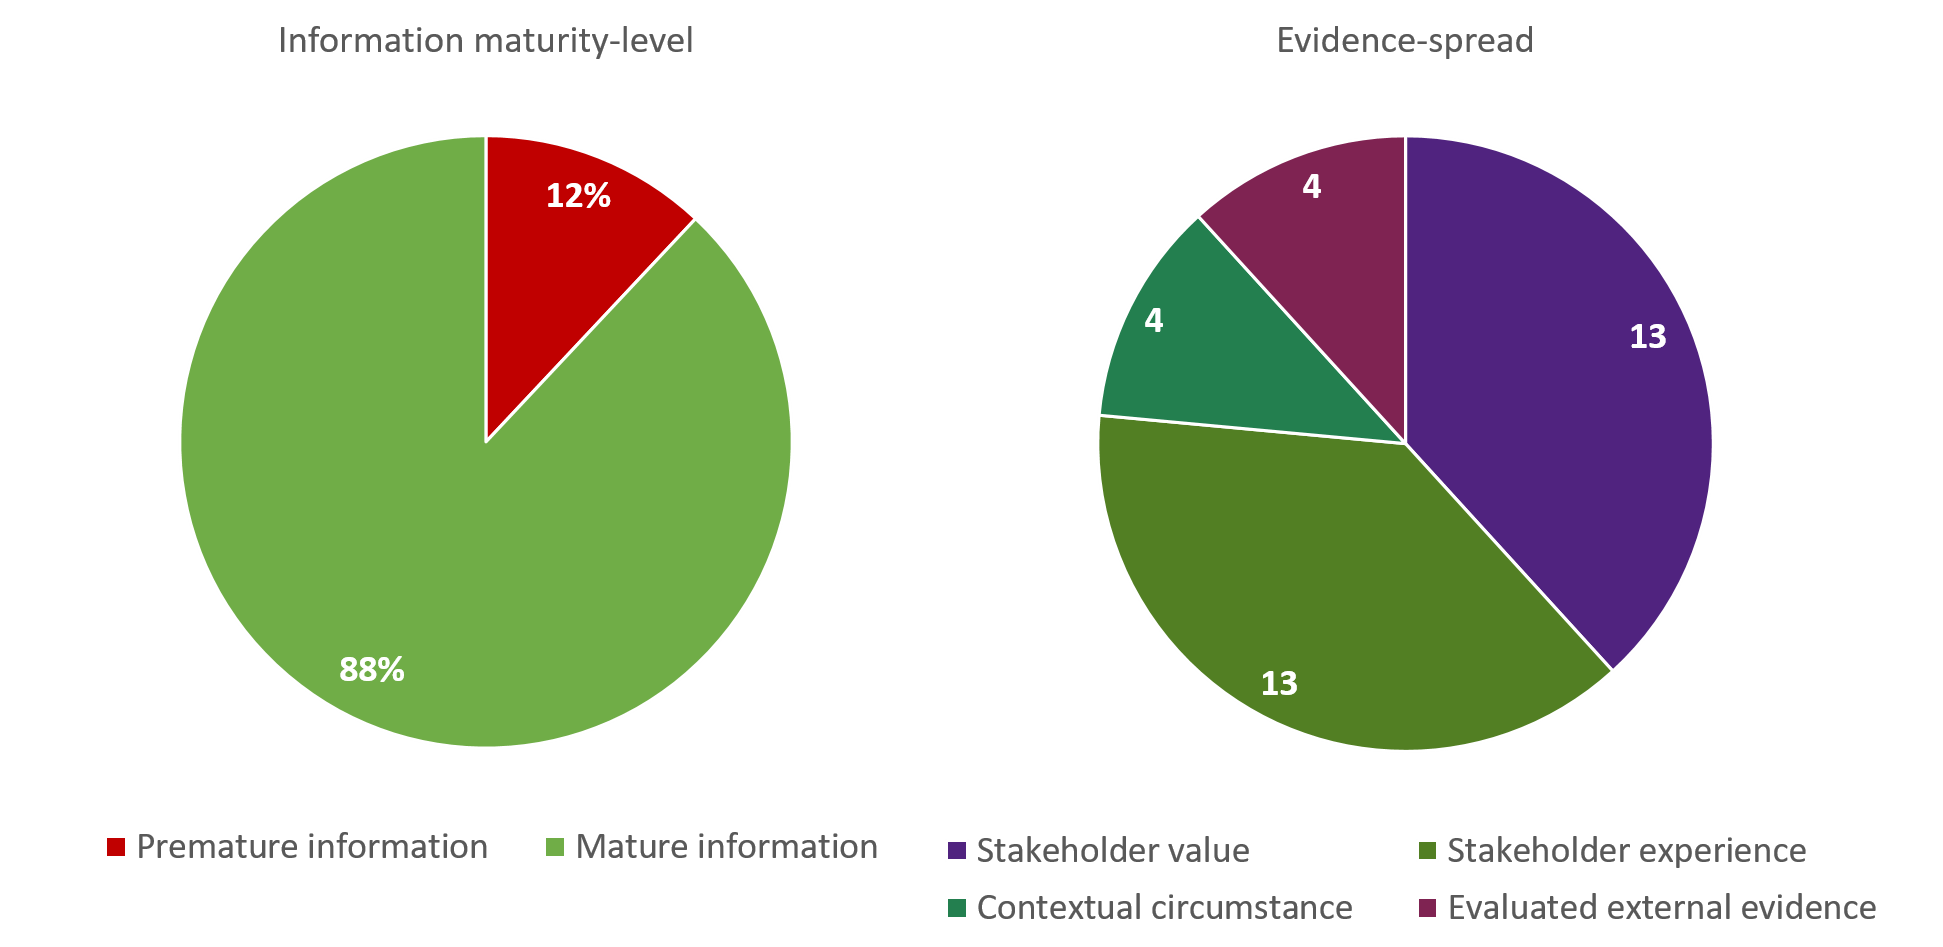
\includegraphics[width=14cm]{../../Images/05_Validation/05_AS_Dashboard_Component_1_AS_DEC1.png}
  \caption{A mock-up of the first decision presentation pattern dashboard for test scenario $DEC1$. The dashboard reflects an information maturity-level of $0.88$ and the evidence spread table \ref{table:as_evidence_spread_DEC1} presents.}
  \label{fig:05_AS_Dashboard_Component_1_AS_DEC1}
\end{figure}

The second dashboard of the decision presentation pattern presents the information maturity-level per pattern. We present the pattern-specific maximum and actual violations in table \ref{table:as_maximum_evidence_dec1}.

The decision-relevant root individuals for $DEC1$ generate completeness violations. These violations match our expectations as scenario $SC2$ validates the completeness pattern. The completeness pattern generates $12$ violations. The other patterns do not generate any violations.

Figure \ref{fig:05_AS_Dashboard_Component_2_AS_DEC1} presents a mock-up of the second decision presentation pattern dashboard. The dashboard reflects the completeness maturity-level of $\dfrac{45-12}{45} = 0.733$, which results in 73\%. The maturity-levels of the other patterns are 100\% as they do not generate any violations.

\begin{figure}[H]
\centering
  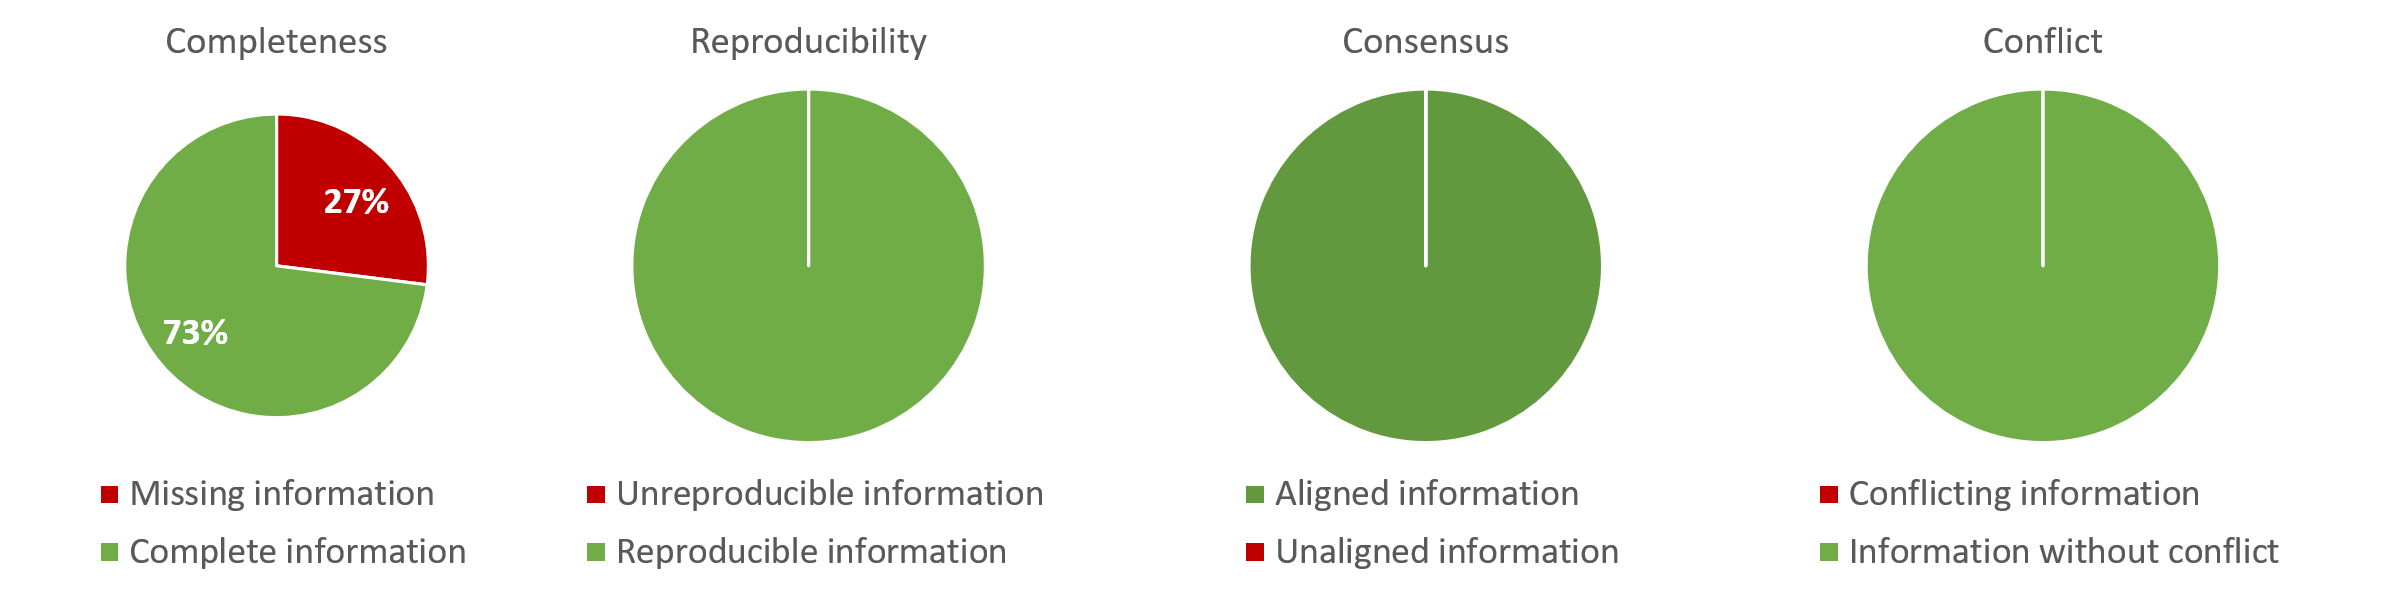
\includegraphics[width=17cm]{../../Images/05_Validation/05_AS_Dashboard_Component_2_AS_DEC1.png}
  \caption{A mock-up of the second decision presentation pattern dashboard for decision $DEC1$.}
  \label{fig:05_AS_Dashboard_Component_2_AS_DEC1}
\end{figure}

To complete the missing information, the software product manager needs to know which information is incomplete. The third dashboard of the decision presentation pattern presents the completeness of information per decision-relevant individual.

Figure \ref{fig:05_AS_Dashboard_Component_3_AS_DEC1_Completeness} presents a mock-up of the third decision presentation pattern dashboard, considering the software product manager selected $System\_SC2$. We observe that five decision-relevant individuals are incomplete. The bar chart gives the software product manager an indication which individuals are causing the 73\% completeness maturity-level. The software product manager wants to know more information on $System\_SC2$. The dashboard presents related violations in the table below the bar chart. The dashboard consolidates the violations of $System\_SC2\_To\_Be$ under $System\_SC2$.

\begin{figure}[H]
\centering
  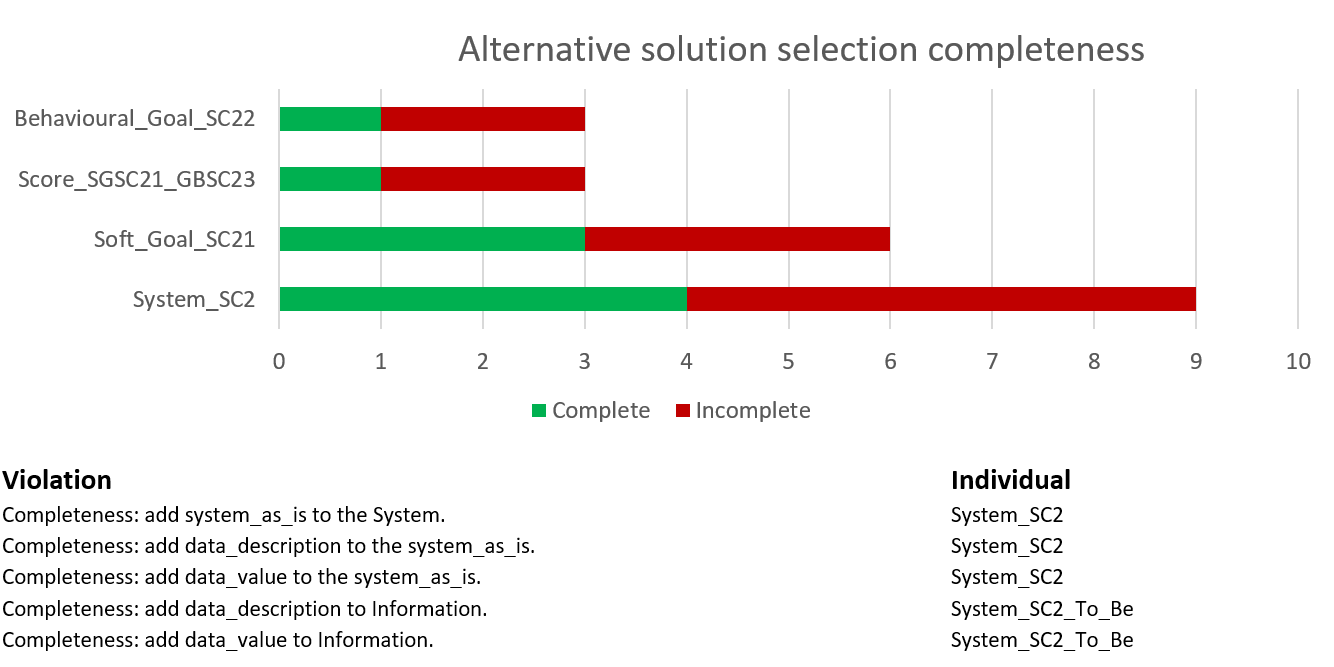
\includegraphics[width=16cm]{../../Images/05_Validation/05_AS_Dashboard_Component_3_AS_DEC1_Completeness.png}
  \caption{A mock-up of the third decision presentation pattern dashboard, considering the decision-maker selected $System\_SC2$. We observe that five decision-relevant individuals are incomplete.}
  \label{fig:05_AS_Dashboard_Component_3_AS_DEC1_Completeness}
\end{figure}
